
\documentclass[a4paper]{article}
\usepackage{ucs}  % unicode
\usepackage[utf8x]{inputenc}
\usepackage[T2A]{fontenc}
\usepackage[bulgarian]{babel}
\usepackage{graphicx}
\usepackage{fancyhdr}
\usepackage{lastpage}
\usepackage{listings}
\usepackage{fancyvrb}
\usepackage[usenames,dvipsnames]{color}
\setlength{\headheight}{12.51453pt}

%%%%%%%%%%%%%% Pygments header.
\makeatletter
\def\PY@reset{\let\PY@it=\relax \let\PY@bf=\relax%
    \let\PY@ul=\relax \let\PY@tc=\relax%
    \let\PY@bc=\relax \let\PY@ff=\relax}
\def\PY@tok#1{\csname PY@tok@#1\endcsname}
\def\PY@toks#1+{\ifx\relax#1\empty\else%
    \PY@tok{#1}\expandafter\PY@toks\fi}
\def\PY@do#1{\PY@bc{\PY@tc{\PY@ul{%
    \PY@it{\PY@bf{\PY@ff{#1}}}}}}}
\def\PY#1#2{\PY@reset\PY@toks#1+\relax+\PY@do{#2}}

\def\PY@tok@gd{\def\PY@tc##1{\textcolor[rgb]{0.63,0.00,0.00}{##1}}}
\def\PY@tok@gu{\let\PY@bf=\textbf\def\PY@tc##1{\textcolor[rgb]{0.50,0.00,0.50}{##1}}}
\def\PY@tok@gt{\def\PY@tc##1{\textcolor[rgb]{0.00,0.25,0.82}{##1}}}
\def\PY@tok@gs{\let\PY@bf=\textbf}
\def\PY@tok@gr{\def\PY@tc##1{\textcolor[rgb]{1.00,0.00,0.00}{##1}}}
\def\PY@tok@cm{\let\PY@it=\textit\def\PY@tc##1{\textcolor[rgb]{0.25,0.50,0.50}{##1}}}
\def\PY@tok@vg{\def\PY@tc##1{\textcolor[rgb]{0.10,0.09,0.49}{##1}}}
\def\PY@tok@m{\def\PY@tc##1{\textcolor[rgb]{0.40,0.40,0.40}{##1}}}
\def\PY@tok@mh{\def\PY@tc##1{\textcolor[rgb]{0.40,0.40,0.40}{##1}}}
\def\PY@tok@go{\def\PY@tc##1{\textcolor[rgb]{0.50,0.50,0.50}{##1}}}
\def\PY@tok@ge{\let\PY@it=\textit}
\def\PY@tok@vc{\def\PY@tc##1{\textcolor[rgb]{0.10,0.09,0.49}{##1}}}
\def\PY@tok@il{\def\PY@tc##1{\textcolor[rgb]{0.40,0.40,0.40}{##1}}}
\def\PY@tok@cs{\let\PY@it=\textit\def\PY@tc##1{\textcolor[rgb]{0.25,0.50,0.50}{##1}}}
\def\PY@tok@cp{\def\PY@tc##1{\textcolor[rgb]{0.74,0.48,0.00}{##1}}}
\def\PY@tok@gi{\def\PY@tc##1{\textcolor[rgb]{0.00,0.63,0.00}{##1}}}
\def\PY@tok@gh{\let\PY@bf=\textbf\def\PY@tc##1{\textcolor[rgb]{0.00,0.00,0.50}{##1}}}
\def\PY@tok@ni{\let\PY@bf=\textbf\def\PY@tc##1{\textcolor[rgb]{0.60,0.60,0.60}{##1}}}
\def\PY@tok@nl{\def\PY@tc##1{\textcolor[rgb]{0.63,0.63,0.00}{##1}}}
\def\PY@tok@nn{\let\PY@bf=\textbf\def\PY@tc##1{\textcolor[rgb]{0.00,0.00,1.00}{##1}}}
\def\PY@tok@no{\def\PY@tc##1{\textcolor[rgb]{0.53,0.00,0.00}{##1}}}
\def\PY@tok@na{\def\PY@tc##1{\textcolor[rgb]{0.49,0.56,0.16}{##1}}}
\def\PY@tok@nb{\def\PY@tc##1{\textcolor[rgb]{0.00,0.50,0.00}{##1}}}
\def\PY@tok@nc{\let\PY@bf=\textbf\def\PY@tc##1{\textcolor[rgb]{0.00,0.00,1.00}{##1}}}
\def\PY@tok@nd{\def\PY@tc##1{\textcolor[rgb]{0.67,0.13,1.00}{##1}}}
\def\PY@tok@ne{\let\PY@bf=\textbf\def\PY@tc##1{\textcolor[rgb]{0.82,0.25,0.23}{##1}}}
\def\PY@tok@nf{\def\PY@tc##1{\textcolor[rgb]{0.00,0.00,1.00}{##1}}}
\def\PY@tok@si{\let\PY@bf=\textbf\def\PY@tc##1{\textcolor[rgb]{0.73,0.40,0.53}{##1}}}
\def\PY@tok@s2{\def\PY@tc##1{\textcolor[rgb]{0.73,0.13,0.13}{##1}}}
\def\PY@tok@vi{\def\PY@tc##1{\textcolor[rgb]{0.10,0.09,0.49}{##1}}}
\def\PY@tok@nt{\let\PY@bf=\textbf\def\PY@tc##1{\textcolor[rgb]{0.00,0.50,0.00}{##1}}}
\def\PY@tok@nv{\def\PY@tc##1{\textcolor[rgb]{0.10,0.09,0.49}{##1}}}
\def\PY@tok@s1{\def\PY@tc##1{\textcolor[rgb]{0.73,0.13,0.13}{##1}}}
\def\PY@tok@sh{\def\PY@tc##1{\textcolor[rgb]{0.73,0.13,0.13}{##1}}}
\def\PY@tok@sc{\def\PY@tc##1{\textcolor[rgb]{0.73,0.13,0.13}{##1}}}
\def\PY@tok@sx{\def\PY@tc##1{\textcolor[rgb]{0.00,0.50,0.00}{##1}}}
\def\PY@tok@bp{\def\PY@tc##1{\textcolor[rgb]{0.00,0.50,0.00}{##1}}}
\def\PY@tok@c1{\let\PY@it=\textit\def\PY@tc##1{\textcolor[rgb]{0.25,0.50,0.50}{##1}}}
\def\PY@tok@kc{\let\PY@bf=\textbf\def\PY@tc##1{\textcolor[rgb]{0.00,0.50,0.00}{##1}}}
\def\PY@tok@c{\let\PY@it=\textit\def\PY@tc##1{\textcolor[rgb]{0.25,0.50,0.50}{##1}}}
\def\PY@tok@mf{\def\PY@tc##1{\textcolor[rgb]{0.40,0.40,0.40}{##1}}}
\def\PY@tok@err{\def\PY@bc##1{\fcolorbox[rgb]{1.00,0.00,0.00}{1,1,1}{##1}}}
\def\PY@tok@kd{\let\PY@bf=\textbf\def\PY@tc##1{\textcolor[rgb]{0.00,0.50,0.00}{##1}}}
\def\PY@tok@ss{\def\PY@tc##1{\textcolor[rgb]{0.10,0.09,0.49}{##1}}}
\def\PY@tok@sr{\def\PY@tc##1{\textcolor[rgb]{0.73,0.40,0.53}{##1}}}
\def\PY@tok@mo{\def\PY@tc##1{\textcolor[rgb]{0.40,0.40,0.40}{##1}}}
\def\PY@tok@kn{\let\PY@bf=\textbf\dthod of a LatexFormatter returns a string containing \def commands ef\PY@tc##1{\textcolor[rgb]{0.00,0.50,0.00}{##1}}}
\def\PY@tok@mi{\def\PY@tc##1{\textcolor[rgb]{0.40,0.40,0.40}{##1}}}
\def\PY@tok@gp{\let\PY@bf=\textbf\def\PY@tc##1{\textcolor[rgb]{0.00,0.00,0.50}{##1}}}
\def\PY@tok@o{\def\PY@tc##1{\textcolor[rgb]{0.40,0.40,0.40}{##1}}}
\def\PY@tok@kr{\let\PY@bf=\textbf\def\PY@tc##1{\textcolor[rgb]{0.00,0.50,0.00}{##1}}}
\def\PY@tok@s{\def\PY@tc##1{\textcolor[rgb]{0.73,0.13,0.13}{##1}}}
\def\PY@tok@kp{\def\PY@tc##1{\textcolor[rgb]{0.00,0.50,0.00}{##1}}}
\def\PY@tok@w{\def\PY@tc##1{\textcolor[rgb]{0.73,0.73,0.73}{##1}}}
\def\PY@tok@kt{\def\PY@tc##1{\textcolor[rgb]{0.69,0.00,0.25}{##1}}}
\def\PY@tok@ow{\let\PY@bf=\textbf\def\PY@tc##1{\textcolor[rgb]{0.67,0.13,1.00}{##1}}}
\def\PY@tok@sb{\def\PY@tc##1{\textcolor[rgb]{0.73,0.13,0.13}{##1}}}
\def\PY@tok@k{\let\PY@bf=\textbf\def\PY@tc##1{\textcolor[rgb]{0.00,0.50,0.00}{##1}}}
\def\PY@tok@se{\let\PY@bf=\textbf\def\PY@tc##1{\textcolor[rgb]{0.73,0.40,0.13}{##1}}}
\def\PY@tok@sd{\let\PY@it=\textit\def\PY@tc##1{\textcolor[rgb]{0.73,0.13,0.13}{##1}}}

\def\PYZbs{\char`\\}
\def\PYZus{\char`\_}
\def\PYZob{\char`\{}
\def\PYZcb{\char`\}}
\def\PYZca{\char`\^}
% for compatibility with earlier versions
\def\PYZat{@}
\def\PYZlb{[}
\def\PYZrb{]}
%%%%%%%%%%%%%% Pygments header end.

\fancyhf{}
\fancyhead{}
\fancyhead[LE,RO]{\thepage\ от \pageref{LastPage}}
\fancyhead[RE]{\textit{\nouppercase{\leftmark}}}
\fancyhead[LO]{\textit{\nouppercase{\rightmark}}}
\pagestyle{fancy}

\addto\captionsbulgarian{%
  \def\abstractname{%
    Цел на проекта} %\cyr\CYRA\cyrs\cyrt\cyrr\cyra\cyrk\cyrt}}%
}

% VCS = Version Control Systems

% Custom defines:
\def\Hg{Mercurial}

% TODO remove colorlinks before printing
\usepackage[unicode,colorlinks]{hyperref}   % this has to be the _last_ command in the preambule, or else - no work
\hypersetup{urlcolor=blue}
\hypersetup{citecolor=PineGreen}

\begin{document}

\title{
Разпределени системи \\
за управление на код
}
\author{
Зорница Атанасова Костадинова, 4 курс, КН, фн: 80227, \\
Искрен Ивов Чернев, 4 курс, КН, фн: 80246
}
\date{\today}
\maketitle

\begin{abstract}
Да запознае читателя с историята и развитието на системите за управление на код
(SCM). Ще бъдат сравнени централизираните и дистрибутираните системи както на
високо ниво - предимства, недостатъци, сфери на приложение - така и на ниско
ниво - обща архитектура, представяне на данните, използвани алгоритми
и структури от данни. Ще бъде обърнато специално внимание на дистрибутираните
системи за управление на код, тъй като те са по-нови като концепция и вече
успешно заместват централизираните системи във все повече проекти,
най-забележимо тези с отворен код, но също и в големи компании които по
исторически причини използват централизирани системи (google, facebook).
\end{abstract}
\newpage

\setcounter{tocdepth}{2}
\tableofcontents
\newpage

%%%%%
%%%%% Templates
%%%%%
% \section{Секция}
% 
% \subsection{Под секция}
% \subsubsection{Под под секция}
% 
% Enumerate list \cite{foo}
% 
% \begin{enumerate}
%   \item първо
%   \item второ
%   \item трето
% \end{enumerate}
% 
% Itemize list
% 
% \begin{itemize}
%   \item Едно
%   \item[Две] 2
%   \item[Триииииииииииииииииииииииииии] три три три три три
%   три три три три
%   \item \texttt{Четири} \\
%     Това е на нов ред
% \end{itemize}
% 
% Description list
% 
% \begin{description}
%   \item[Foo] bar
%   \item[баз] quux
% \end{description}
%
% \footnote{this is a footnote}
%
% \cite{citation} % put it in bibliography at the bottom of the doc
% \begin{thebibliography}{99}
%   \bibitem{citation} \url{http://example.com/}
% \end{thebibliography}
%
% ``quotation''

% \label{markThisSpot}
% use the reference like that:
% \ref{markThisSpot} is located on page \pageref{markThisSpot}
% 

%%%%%% Begin of document (BOD)

\section{Увод}
Системите за управление на код (SCM) играят важна роля в процеса на
разработване на софтуер. Те съхраняват историята на развитие на файловете като
по този начин позволяват на потребителя да прегледа направените промени по
различни критерии (времеви период, потребител направил промяната).
Правенето на промени по кодовата база също е благоприятствано от факта, че те
винаги могат да се игнорират и състоянието на проекта да бъде върнато към
предишно стабилно такова. Историята на развитие на проекта може да бъде
използвана и от хора интересуващи се от прогреса по проекта (мениджъри,
клиенти), с цел създаване на план за по-нататъшно развитие и оценка за свършена
работа.


Софтуерните проекти обикновено се развиват в няколко направления:
\begin{itemize}
  \item едно или няколко стабилни направления - използват се от обикновения
  потребител;
  \item направление за тестване (beta версия) - използва се от по-напреднали
  потребители, които искат да получат нововъведенията колкото се може по-скоро,
  дори на цената на по-нестабилно поведение;
  \item направление за развитие - използва се от програмистите докато
  разработват най-новите промени по кода.
\end{itemize}


SCM предоставят възможности за управление на отделните направления като по
този начин може да се разграничи кои версии от историческото развитие се
използват от програмисти, от тестери и от обикновени потребители.

\section{История и развитие на SCM}
Нуждата от SCM се появява през 60\textsuperscript{те} и
70\textsuperscript{те} години на XX век. През
това време се появяват първите по-големи софтуерни проекти и става ясно, че
поддържането на историята на развитие на проекта е крайно наложително.
Развитието преминава през няколко периода:
  \subsection{Ръчно управление}
  В началото всеки сам е решавал проблема с пазене на история на проект или
  отделен файл. Нужен е бил механизъм за запаметяване на състоянието на един
  или няколко файла в даден момент, за да може при нужда да се върне старо
  състояние. Това може да става със запазване на стара версия на файла с
  различно разширение (например \texttt{filename.old.1},
  \texttt{filename.old.2} и т.н.) или създаване на архив на цяла директория.
  Тези подходи вършат работа при малки начинания, но имат големия недостатък, че
  изразходват много памет. Ако един файл има дължина 1 Kb и е бил запазен 20
  пъти от момента на своето създаване, тогава заеманата памет е приблизително
  $1000 * 20 / 2 = 10 \mathrm{Kb}$. Това означава, че необходимата памет нараства
  линейно с броя на запаметените ревизии. На практика обаче всяка
  ревизия се различава с малко от предходната. Това означава, че независимо от
  броя на ревизиите заеманата памет теоретично би могла да бъде пропорционална 
  на размера на проекта.

  \subsection{Локално управление}
  Първите софтуерни продукти за управление на код са работели на ниво отделен
  файл. Запазвали са историята на един файл независимо от останалите.  Това
  може да бъде постигнато като за всяка нова ревизия бъде запазена разликата
  с предишната. Първата система, която реализира това е SCCS\footnote{Source
  Code Control System\cite{sccs}}. Тя използва механизмът на припокриващи се
  разлики (interleaved deltas) за да запази различията между версиите на един
  файл. Системата е била разработвана от Bell Labs и се разпространявала чрез
  заплащане. RCS\footnote{Revision Control System\cite{rcs}} е наследник на
  SCCS и набрала голяма популярност през 80\textsuperscript{те} години, защото
  била безплатен и усъвършенстван еквивалент на SCCS. RCS също предоставяла
  възможност за следене на история на всеки файл по отделно. Освен работната
  версия на файла се пазел и файл с историята, съдържащ списък с промените
  приложени върху файла от началното до крайното му състояние.

  \subsection{Централизирано управление} Представените до момента системи дават
  възможност за пазене на историята на отделни файлове на компютъра на който са
  били създадени. Възникнала необходимостта тази история да се предоставя на
  група хора - екип програмисти. Разпределянето на файла с историята между
  няколко компютри се оказало нелека задача, особено при наличието на много
  файлове. Нужна била система която е в състояние да управлява всички файлове
  на проекта и да осигури лесен и бърз начин за достъпване на историята на
  проекта от всеки член на екипа. С тези идеи била създадена
  CVS\footnote{Concurrent Versions System\cite{cvs}} - една от най-известните
  системи за управление на код, използвана и в момента от немалко проекти.
  В нея точно както в RCS е имплементирано запазването на история за всеки
  файл. Присъства и централен сървър на който стои информация за историята на
  всички файлове. При клиента се намира само една текуща версия на всички
  файлове и при нужда от други версии той се свързва със сървъра и изтегля
  нужната му информация. За да поправи много от проблемите открити с времето
  в CVS бил създаден Subversion\cite{svn}. Subversion има мото ``CVS направен
  както трябва''. Тъй като решава доста проблеми на CVS и е лесен за използване,
  много проекти мигрират от CVS на Subversion. При Subversion се запазва идеята
  за един централен сървър с който потребителите се свързват и актуализират
  файловете си.

  \subsection{Разпределено управление}
  Най-същественото различие на дистрибутираните системи за управление на код
  спрямо централизираните е, че всеки клиент притежава на локалната си машина
  пълната история на развитие на проекта.  Тъй като всеки добавя сам нова
  история трябва да съществува механизъм за обмяна на промените направени между
  самите клиента. Това означава, че може лесно да се наподоби моделът на работа
  на централизираните системи като се избере един централен клиент и останалите
  се синхронизират с него. На практика се използва както централен клиент, така
  и синхронизиране на два нецентрални клиента, в зависимост от ситуацията.
  
  Най-известните примери за разпределени системи за управление са
  Git\cite{git} и Mercurial\cite{mercurial}. Те набират голяма популярност
  сред open source обществото защото улесняват споделянето на промени между
  хора, които не се познават и следователно нямат общ централен сървър.

\section{Сравнение на архитектурно ниво}

  \paragraph{Модел за едновременен достъп}
  Описва как в случай на едновременна редакция на файлове се избягва въвеждането в хранилището на неверни данни.
  \begin{itemize}
    \item \texttt{Схема със заключване} -- Промени не са позволени докато потребителят не поиска и получи изключителните права над файла от основното хранилище. Файлът е заключен докато трае текущата редакция.
    \item \texttt{Схема със сливане} -- Потребителите са свободни да редактират всички файлове, но при опит да добавят промените си в хранилището са информирани за евентуалните конфликти. В такъв случай системата за контрол на версиите може да разреши конфликта или ако не успее да остави потребителят сам да го разреши.
  \end{itemize}
  Разпределените системи почти винаги предполагат моделa със сливане.




  \subsection{Архитектура на централизираните системи}
    \subsubsection{Архитектура на CVS}

    CVS (съкратено от Concurrent Versions System) е една от първите широко
    достъпни системи за управление на код с клиент-сървър архитектура. Сървърът
    пази информация за цялата история на всички файлове от проекта, а клиентът
    може да свали произволна версия от сървъра (check-out), да направи локални
    промени, след което да качи промените на сървъра (check-in).

    Системата е паралелна (concurrent) защото позволява на произволен брой
    програмисти да работят едновременно -- да правят промени върху един
    и същ проект по едно и също време. Единственото условие е при check-in
    между последния check-out да няма check-in на друг потребител. Ако
    версията свалена от сървъра е най-новата и не се появи по-нова заради
    check-in на друг качването е успешно. Ако някой друг е създал нова
    версия междувременно, то останалите трябва първо да свалят новата последна
    версия, да обединят промените си с нея и да след това да запишат своите
    промени. В повечето случаи тази операция се извършва автоматично от CVS.
    Проблем създават само ситуациите при които е редактиран един и същи файл на
    еднакви места -- тогава се налага намесата на програмиста.

      \paragraph{Запазване на историята}

      Историята на файловете в CVS repository се запазва за всеки файл по
      отделно, като се използва RCS формат -- списък с промените довели от
      началното до крайното състояние. Когато се създава нова версия файловете
      които са променени увеличават своята версия (промяната им се записва
      във файла с историята). Файловете участващи във всяка версия не са
      групирани по никакъв начин. Това е проблем ако искаме да видим
      състоянието на проекта във фиксиран минал момент -- всеки файл пази
      своята история, но информацията за това кои версии на файловете са
      свързани в ревизиите на целия проект липсва. Това налага ръчното
      маркиране на ревизии със специални имена, за да може лесно да се
      възстанови исканото предишно състояние на всички файлове.

      \paragraph{Връзка със сървъра}

      При качване на промени към сървъра е възможно част от файловете да бъдат
      обновени, а останалите не -- например при липса на стабилна мрежовата
      свързаност. Това създава проблеми, защото в по-голям проект със сигурност
      ще се случи, оставя хранилището в несъвместимо състояние, а поправянето
      става единствено ръчно от администратора.

    \subsubsection{Архитектура на Subversion}
    
\includegraphics[scale=1.0]{svn_icon}
    
    Apache Subversion (или само SVN по името на командата svn) е система за
    контрол на версиите създадена с цел да бъде силно подобна на CVS,
    поправяйки грешките и имплементирайки някои липсващи нейни функционалности.
    Използва се широко в средите почитащи отворения код. Сред примерите са
    Apache Software Foundation, FreeBSD, GCC, Django, Ruby, Tigris.org, PHP,
    Python и MediaWiki. Google Code и SourceForge предоставят Subversion
    хостинг за проекти с отворен код.

    Функционалности, които го правят предпочитан пред CVS:
    \begin{itemize}
      \item \texttt{Атомарни commit-и} - В смисъла на транзакциите. Или цялото множество от промени се регистрира, или абсолютно нищо.
      \item \texttt{Пълна история} на преименовани, копирани или преместени файлове и директории.
      \item \texttt{Метаданни} - Може да се съхранява информация за файлове и директории под формата на двойки ключ - стойност.
      \item \texttt{Двоични файлове} - Съхранението им е ефективно, като от ревизия до ревизия се пази само binary-diff.
      \item \texttt{Branching} e евтина операция независеща от размера на файловете. Механизмът е подобен на хард-линковете в UNIX.
      \item \texttt{Обмен на малко информация} - Протоколът между клиента и сървъра изпраща само diff'ове на файловете в двете посоки.
      \item \texttt{Резултатите} са удобни за парсене. Има възможност за получаване на лог във вид на XML.
      \item \texttt{Конфликти} - За да се избегне необходимостта от разрешаване на конфликти, файловете могат да се заключват. Така програмистът си запазва изключителното право само той да ги редактира (reserved checkout).
      %\item Path-based authorization.
      \item \texttt{Интеграция} - SVN е написан на C, но поддържа интеграция също със C\#, PHP, Python, Perl, Ruby и Java.
    \end{itemize}

    \paragraph{Архитектура}
    Моделът е клиент-сървър, дизайнът на библиотеките е слоест.

    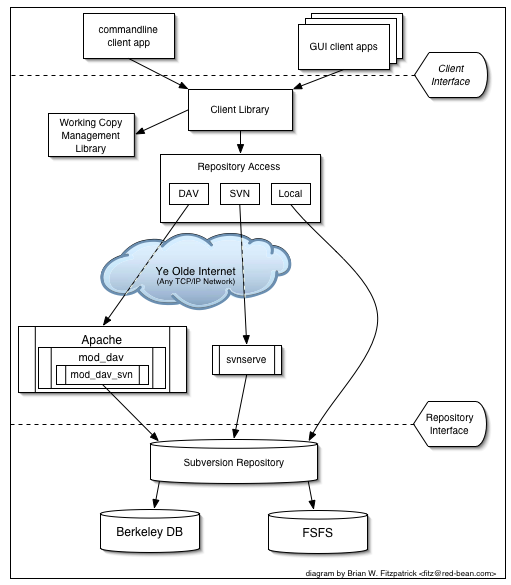
\includegraphics[scale=0.5]{svn_architecture}

    В долната част на схемата се намира SVN repository-то което съдържа всички
    данни регистрирани за контрол на версиите. В горната част е представена
    клиентската програма която управлява локалните копия на тези данни
    (наречени работни копия). Помежду им са множество маршрути през различни
    слоеве за достъп до хранилището. Някои от тях минават през мрежата и през
    сървъри, които от своя страна вземат данните от централния сървър. Други
    нямат нужда да използват мрежата и директно достъпват хранилището.

    \paragraph{Видове хранилища}

    \begin{itemize}
      \item \texttt{Berkeley DB}
      \item \texttt{FSFS} - Предпочитаният метод за съхранение на данните, тъй като работи по-бързо и заема по-малко място на диска.
    \end{itemize}

    \paragraph{Достъп до хранилищата}

    \begin{itemize}
      \item \texttt{Местна или мрежова файлова система} - Използва протокола file:///path.
      \item \texttt{WebDAV / Delta-V} - Чрез модула mod\_dav\_svn за Apache. Протоколът е http(s).
      \item \texttt{Специализиран svn протокол} - Предава обикновен текст (svn://host/path) или криптиран през ssh (svn+ssh://host/path).
    \end{itemize}

    \paragraph{Клиенти}

    \begin{itemize}
      \item В командния ред
        \begin{itemize}
          \item Subversion предоставя собствен клиент за командния ред.
        \end{itemize}
      \item В мениджъра на прозорците
        \begin{itemize}
          \item TortoiseSVN е разширение на Windows shell което информира за състоянието на файловете в revision системата като модифицира иконите в Windows Explorer.
          \item SmartSVN работи на подобен принцип.
        \end{itemize}
      \item Интегрирани в средата за разработване на код
        \begin{itemize}
          \item AnkhSVN е предвидена за ползване с Microsoft Visual Studio.
          \item Subclipse, Subversive работят заедно с Eclipse.
          \item Xcode е редактор, включен в Mac OS X 10.5 (Leopard), поддържащ SVN.
        \end{itemize}
      \item Уеб-базирани
        \begin{itemize}
          \item Trac - вдъхновена е от CVSTrac и първоначално е наречена ``svntrac'' заради интеграцията си със Subversion.
        \end{itemize}
    \end{itemize}

    \paragraph{Слоеве}

    \begin{itemize}
      \item \texttt{Файлова система} -- Това е най-ниското ниво на което се
      съхраняват потребителските данни.
      \item \texttt{Хранилище} -- Контролира скриптовете които изпълняват действията по
      контрол на версиите. Тези два слоя заедно съставляват интерфейса на
      файловата система.
      \item \texttt{mod\_dav\_svn} -- Осигурява WebDAV / Delta-V достъп чрез Apache 2.
      \item \texttt{Достъп до хранилището} -- Този слой контролира както местния
      така и отдалечения достъп. На това ниво към хранилищата се обръщаме чрез
      URL:
        \begin{itemize}
          \item \texttt{местен достъп}: \texttt{file:///path/}
          \item \texttt{WebDAV}: \texttt{http://host/path/} \quad \texttt{https://host/path/}
          \item \texttt{протокол SVN}: \texttt{svn://host/path/} \quad \texttt{svn+ssh://host/path/}
        \end{itemize}
      \item \texttt{Клиент, Работно копие на проекта} -- Най-високото ниво абстрахира
      достъпа до хранилището и предоставя интерфейс за общи клиентски задачи
      като автентикация на потребители и сравнение на версии.
    \end{itemize}

  \subsection{Архитектура на дистрибутираните системи}

    \subsubsection{Архитектура на \Hg}
    
\includegraphics[scale=1.0]{hg_icon}

    \paragraph{Обща информация}
    \Hg\ е многоплатформена, дистрибутирана система за управление на код. Тя
    е написана главно на Python, но съдържа алгоритъм за двоично
    запазване на разликите разработен на C. \Hg\ работи на всички основни
    операционни системи: Windows, Unix-like---Linux, OS X, *BSD. При
    разработването на \Hg\ основни цели са били:
    \begin{itemize}
      \item производителност
      \item скалируемост
      \item децентрализация
      \item пълна дистрибутираност
      \item с адекватно обработване на текстови и двоични файлове
      \item развити средства за разклоняване и сливане
      \item идейно проста
    \end{itemize}

    \paragraph{Основни концепции}
    \subparagraph{revlog}
    \Hg\ пази историята на всеки файл в \texttt{revlog} файлове---един индекс,
    и един за данни. Във файла с данни са записани последователни разлики, или
    целия файл като се преценява какъв обем данни ще са необходими, за да се
    възстанови ревизията при нужда---както видео кодерите запазват цял фрейм,
    последван от няколко разлики с предишния фрейм. Данните се компресират, ако
    компресирания вариант е по-малък от оригинала. В индекс файла са записани
    местата във файла с данни в който започва описанието на всяка нова версия
    (било то разлика с предходната или целия файл), заедно с мета данни.

    Всяка ревизия на всеки файл има уникален идентификатор наречен
    \texttt{nodeid}. Той се получава като се сметне SHA1\cite{sha1} сумата на файла,
    слепен с \texttt{nodeid}-то на предишната версия на файла. Това гарантира,
    че всеки файл в процеса на своето създаване ще получава винаги различни
    \texttt{nodeid} за различните си версии, даже съдържанието на файла да
    е напълно еднакво.
    \vspace{5 mm}

    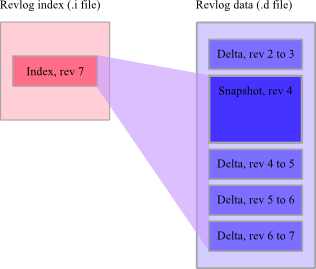
\includegraphics[scale=0.7]{hg_revlog}

    \subparagraph{manifest} Информацията за това кои версии на всеки файл
    участват във всяка отделна ревизия на проекта се запазва в manifest файл.
    Една и съща версия на файл може да участва в няколко последователни версии
    на manifest-а, ако файла не е бил променян в тези ревизии на проекта.
    Информацията се пази в двоичен формат и представлява \texttt{nodeid} на
    версията на файла заедно с пълното му име. Тъй като manifest-а е файл,
    който се променя с времето различните му ревизии се пазят в revlog---т.е
    точно както се пазят промените в нормалните файлове. Това е удачно, тъй
    като големи части от manifest файла сочат към едни и същи версии на
    файловете, защото сравнително малко файлове биват променени при всяка нова
    версия на целия проект. Така последователните ревизии на манифеста се
    различават с малко, което значително намалява необходимата памет за
    запазване на всички версии.

    \subparagraph{changelog}
    Информацията за самите ревизии на проекта се съхраняват в changelog.
    Информацията включва дата, потребител направил ревизията, предишна
    ревизия (ревизии в случай на сливане), списък с променените файлове
    и \texttt{nodeid} на manifest файла, съдържащ информация за файловите
    версии на тази ревизия. changelog файла също се пази в revlog формат.

    \vspace{10 mm}

    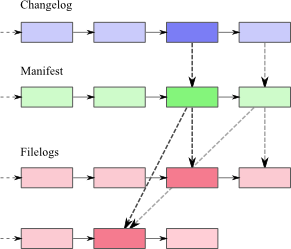
\includegraphics[scale=1.0]{hg_basics}

    \subparagraph{dirstate}
    Състоянието на текущата директория се пази в dirstate. То се използва при
    записване на промените при създаване на нова ревизия. Пази се кога за
    последно \Hg\ е променял всеки файл и колко е бил размера на файла в този
    момент. Когато потребителя се интересува от състоянието на работната
    директория (посредством \texttt{hg status}) \Hg\ проверява последното време
    на промяна на всеки файл в проекта и го сравнява с информацията в dirstate.
    Ако съвпада, тогава се приема, че файла не е бил променян. Ако не съвпада
    се гледа текущия размер на файла. Ако размера е различен---то файла е бил
    променен, само в противен случай се налага сравняване на целия файл
    с последната ревизия запазена от \Hg.

    \paragraph{Начин на работа}
    Когато се наложи да се разгледа състоянието на проекта в определена
    (вероятно минала) ревизия---например с командата \texttt{hg update} се
    случват следните неща:
    \begin{enumerate}
      \item прочита се индекс файла на changelog и се намира мястото в data
      файла където стои информация за дадената ревизия на changelog-a
      \item възстановява се желаната ревизия от changelog data файла---това
      включва акумулирането на няколко разлики върху пълна версия---всички взети
      от data файла
      \item прочита се nodeid на manifest-а от changelog за съответната версия
      \item възстановява се manifest-а със съответното nodeid---пак чрез
      използване на index и data файловете му
      \item от manifest-а се взима информация за nodeid на всички файлове
      участвали в проекта за фиксираната версия
      \item от index и data файловете за всеки файл посредством nodeid се
      възстановяват и самите файлове и се записват в текущата работна
      директория
    \end{enumerate}

    \paragraph{Разклонения и сливания}
    Основна разлика между дистрибутираните и централизираните системи
    е лекотата с която дистрибутираните се справят с разклоненията и сливанията
    в проекта. При централизираните системи всяка ревизия на проект има точно
    една предишна---което означава, че проекта се развива праволинейно. При
    дистрибутираните системи е често срещано много хора едновременно да работят
    върху една и съща начална ревизия (това е разклонение). Това означава, че
    всички техни промени няма да включват промените на всички останали. Това се
    случва често и следователно е нужен механизъм по който да бъдат обединени
    различните промени, за да се получи версия на проекта, в която всички
    промени са извършени (това е сливане).

    В \Hg\ всяка ревизия на проекта може да има един или два предшественика.
    Само един предшественик означава, че върху някаква ревизия са направени
    промени и така се е образувала нова ревизия (повечето ревизии в един
    стандартен проект са точно такива). При наличие на ревизии с по един
    предшественик е възможно дървото на ревизиите да се разклони---ако две
    промени са базирани на една и съща начална ревизия. За да се слеят две
    ревизии, които споделят обща бащина ревизия се използва нова ревизия с два
    предшественика. На базата на графа на ревизиите \Hg\ успява да слее повечето
    файлове без нужда от човешка намеса, защото има възможността да види какви
    промени са правени по пътя на първия предшественик, и какви промени са
    правени по пътя на втория предшественик до най-близката обща ревизия. Ако
    промените са по не пресичащи се части от файла може да бъде направено
    автоматично сливане. Ако промените засягат едни и същи части на един
    файл---например по едната верига е изтрит даден ред, а в другата
    е модифициран се налага потребителя да редактира файла на ръка.

    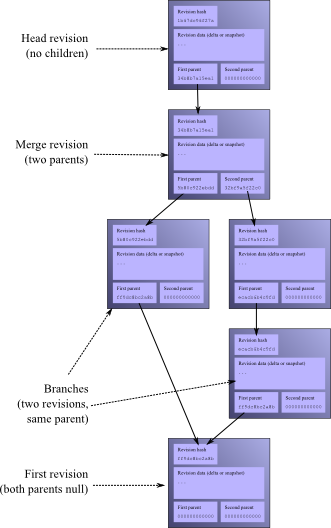
\includegraphics[scale=0.5]{hg_revisions}

    \paragraph{Компресия}
    Когато \Hg\ запазва файлове на диска се използва deflate\cite{deflate}
    алгоритъма, който дава добър баланс между използвано място и време за
    (де)компресиране. Ако обаче се предават данни по мрежата компресираното
    съдържание се декомпресира, след което се компресира на ново с друг
    алгоритъм, който е по-бавен но и по ефективен. Компресира се целия поток от
    данни което е по-ефективно по време и памет, от компресиране на отделните
    файлове. Ако за преноса на данни се използва \texttt{ssh}\cite{ssh}, то
    данните въобще не се компресират, защото \texttt{ssh} има вградена
    поддръжка за компресиране. С това \Hg\ постига по-добра ефективност върху
    повече видове мрежи.

    \paragraph{Нареждания на входно/изходните операции и атомарност}
    \Hg\ гарантира, че клиент четящ от repository-то никога няма да види
    частични данни, въведени от клиент който пише във същия момент. Това
    означава, че във всеки един момент може да има един пишещ клиент и много
    четящи, което значително подобрява времето за достъп. За да се постигне
    това се използват няколко техники.
      \subparagraph{файловете се дописват само в края}
      Както вече стана ясно цялата информация в едно repository се съхранява
      в множество revlog файлове. Записването на нова информация в тях (
      добавянето на нова ревизия) е позволено да се извършва само в края на
      файла. Това подобрява производителността (над методи презаписващи цялото
      съдържание) и улеснява гарантирането на атомарни операции.

      \subparagraph{подреждане на входно/изходните операции}
      Когато се записва нова ревизия на проекта реда на записване е следния:
      \begin{itemize}
        \item записват се revlog data файловете на променените файлове от проекта
        \item записват се revlog index файловете на променените файлове от проекта
        \item записва се revlog data файла на манифеста
        \item записва се revlog index файла на манифеста
        \item записва се revlog data файла на changelog
        \item записва се revlog index файла на changelog
      \end{itemize}
      Както показахме по-горе реда при четене е обратен---това означава, че ако
      в даден момент клиент четящ repository-то прочита данни сочещи (чрез
      nodeid) към вече написани данни в следващия файл.

      \subparagraph{едновременен достъп}
      Подреждането на входно/изходните операции гарантира, че четящ потребител
      няма нужда да заключва repository-то. Това означава, че четящите
      потребители имат само нужда от права за четене. Това значително улеснява
      администрирането на repository-то.

      Пишещите клиенти трябва да заключват repository-то. Механизмът за
      заключване работи на всякакви файлове системи, включително NFS\cite{nfs},
      която по принцип създава всевъзможни проблеми за това. Ако пишещ клиент
      завари заключено repository, той изчаква определено време, проверявайки
      периодично дали се е отключило. Ако времето изтече и repository-то още
      е заключено процеса завършва с неуспех. Това е полезно, ако са настроени
      скриптове които изпълняват периодичен запис -- няма начин нещо да забие
      и акумулиращите чакащи за запис скриптове да изразходят ресурсите на
      системата.

    \subsubsection{Архитектура на Git}
    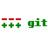
\includegraphics[scale=1.0]{git_icon}

    % TODO(zori): Move images around and scale appropriately.
    % 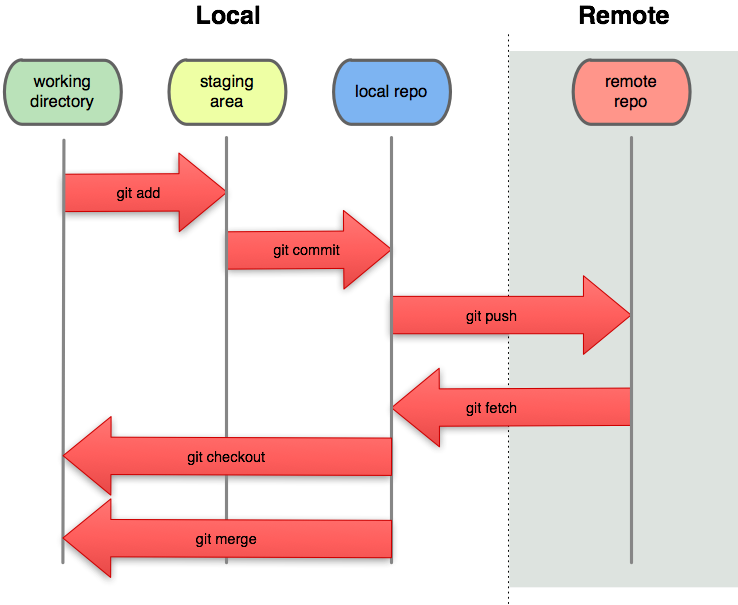
\includegraphics[scale=1.0]{git_everthing_is_local.png}

    Git е създадена от Линус Торвалдс за целите на разработването на ядрото на операционната система Линукс. При писането ѝ се е обърнало специално внимание на скоростта и лесното включване на код от много участници в проекта. Всяка работна директория в Git е пълноправно хранилище с пълна история и възможности за преглеждането ѝ и независима от мрежови достъп до централен сървър.
  
    \paragraph{Дизайн}

    Вдъхновен от BitKeeper и Monotone, Git е бил замислен като engine за система за контрол на версиите на ниско ниво. Над него други щели да надграждат front-end. Проектът обаче се развил дотолкова, че е напълно функционален и за директна употреба. Създателят на Git Линус Торвалдс има широки познания върху работата на файловите системи и опит с поддръжката на голям разпределен проект какъвто е операционната система Линукс. Това предопределя следните решения:

    \begin{itemize}
      \item \texttt{Разпределена разработка} -- Git предоставя на всеки разработчик местно копие на цялата база. Промените се включват от едно хранилище в друго като нови разклонения, които могат да бъдат слени по същия начин като местните разклонения.
      \item \texttt{Ефективност при работа с големи проекти} -- По думите на създателя си Git е бърз и скалируем. Тестове проведени от Mozilla доказват, че е в пъти по-бърз от повечето системи за контрол на версиите, а достъпът до историята на ревизиите от местното хранилище е 2 пъти по-бърз отколкото от отдалечен сървър. Git не става по-бавен с увеличаването на базата от код или акумулираната история на ревизиите.
      \item \texttt{Сериозна поддръжка при не-линейна разработка} -- Важно допускане при дизайна на Git е, че една промяна по-често ще бъде включвана към проектите на участниците отколкото редактирана. Системата поддържа бързо разклоняване и сливане на код и предоставя инструменти за визуализиране и управление на сложна история на разработка.
      \item \texttt{Съвместимост с протоколи и системи} \\
        Медия
        \begin{itemize}
          \item \texttt{ssh}
          \item \texttt{sockets}
        \end{itemize}
        Протоколи
        \begin{itemize}
          \item \texttt{http}
          \item \texttt{ftp}
          \item \texttt{git}
          \item \texttt{rsync}
        \end{itemize}
        Други системи
        \begin{itemize}
          \item \texttt{cvs} Git има възможност за емулиране на CVS сървър и позволява достъпа до хранилища чрез съществуващи cvs клиенти и плъгини за среди за разработка.
          \item \texttt{svn} Съществуващи subversion хранилища могат да се достъпват с командата git-svn.
        \end{itemize}
      \item \texttt{Криптографска автентикация на историята} -- Името на всеки commit зависи от пълната история довела до него. Веднъж направен commit-а не е възможно промяна да не се отрази на криптографския хеш, а следователно и на името на ревизията. В този смисъл промените по Git са immutable.
      \item \texttt{Модулен дизайн} -- Git е създаден като множество програми на C, свързани с shell скриптове - wrapper-и около тези програми. Макар и сега повечето от скриптовете да са пренаписани на С като част от усилието да се направи Git напълно функционален под Windows, дизайнът е останал, което прави лесно навързването и замяната на отделни компоненти.
      \item \texttt{Стратегиите за сливане са лесно заменими} -- Като част от модулния дизайн, Git ясно дефинира незавършено сливане и има множество алгоритми за справяне с него. В случай на невъзможност да се слеят автоматично промените е необходима ръчна редакция от страна на потребителя.
      \item \texttt{BitKeeper като модел} -- Използваната в първите години на разработване на Линукс ядрото система е модел за интерфейса и потока на действия в Git. Технически двете са много различни, което е била една от целите които създателят на Git си е поставил за да бъде очевидно, че макар и създаден да го замести, Git не е копие на BitKeeper.
      \item \texttt{CVS като анти-модел} -- Централизираната система се оказва неприложима за целите на Линус.
      \item \texttt{Сигурност} -- Гаранции срещу повреда на данните, била тя случайна или злонамерена.
    \end{itemize}

    \paragraph{имплементация}
      
      \subparagraph{blob}
      Всички файлове в едно Git repository се представят вътрешно чрез blob.
      Най-важният атрибут на един blob е неговата SHA1 сума. Ако два blob-а
      имат една и съща SHA1 сума repository-то ще го запази точно веднъж.
      В blob се намира само съдържанието на файла. Това означава, че два файла
      с различно име имащи еднакво съдържание ще се представят вътрешно като
      точно един blob.

      \subparagraph{tree}
      Директориите се пазят в структура наречена tree. Тя съдържа информация за обектите които се съдъжат в нея -- списък от тип на обекта, SHA1 сума и име. В tree обектите се помещават други tree обекти и blob-ове.

      \subparagraph{commit}
      Създаването на нова ревизия на проекта се отбелязва в commit обект. Той съдържа:
      \begin{itemize}
        \item SHA1 сумата към главната директория на проекта (tree обект)
        \item SHA1 суми на предшестващи commit обекти -- в случай на сливане е повече от един
        \item информация за автора на ревизията
        \item информация за човека създаващ ревизията в самото repository
        (различен е от автора ако например е получил patch от него и в момента
        го записва като нова ревизия)
        \item съобщение за новата ревизия
      \end{itemize}

      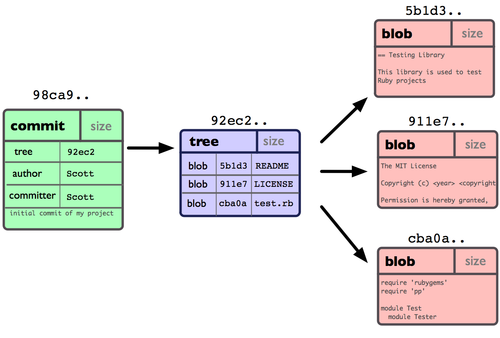
\includegraphics[scale=1.0]{git_commit.png}

      \subparagraph{разлики vs snapshot} За разлика от почти всички останали
      системи за управление на код Git разглежда отделните ревзии на проекта
      като съвкупност от файловете и директориите -- аналогията е да се пази
      архив на главната директория за всяка отделна версия. Останалите системи
      опитват да използват умни алгоритми за следене на файлове по отделните
      ревзии, като запазват или пълната им версия, или разликата с предходната.
      На практика следенето на разликите на ниво файл не винаги е достатъчно --
      ако няколко реда се преместят от един файл в друг в единия файл ще са
      записани като изтрити, а в другия като добавени, но физическа връзка
      между тях никога няма да съществува. В Git промените се засичат на ниво
      repository от сложни евристични алгоритми и на теория могат да се справят
      с проблемите възникващи от per file следене на промени.

      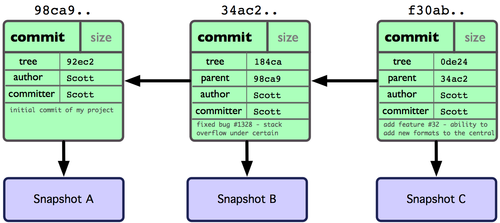
\includegraphics[scale=1.0]{git_commits.png}

      \subparagraph{запазване на blob обекти}
      Git запазва blob обектите по два начина -- неопакован и опакован. При
      неопакования вариант всеки blob се архивира и записва върху диска като
      отделен файл. Това е стандартния начин по който се запиват всички blob
      обекти при нормална работа с repository-то. Това прави git толкова бърз
      -- не се налага да се изчисляват разлики с предишни версии и да се
      акумулират при поискване на определена версия. Ако продължително се
      използва repository-то то ще увеличи много размера си. За да се справи
      с този проблем Git въвежда команда с която се оптимизира размера
      (\texttt{git gc}). Тя прилага сложни евристични алгоритми за да намери
      добър компромис между заето място и време за достъпване. За намаляване на
      размера се използват разлики с предишни версии (точно както почти всички
      други системи). Разликата е, че в Git това не е основен идиом
      а е по-скоро оптимизация, която се прилага само при нужда от алгоритъм,
      имащ информация за всички файлове и ревизии, а не само един файл. На
      практика с тази допълнителна информация алгоритъма може да се справи
      много по-добре.

      \subparagraph{staging area}
      Staging area или index е мястото където се
      записват промените преди те да бъдат записани като нова  ревизия. Това
      е различно от работната директория, която съдържа файловете, с които
      потребителя работи. Това е полезно в случаи в които потребителят
      е направил няколко логически несвързани промени в работната си директория
      и на края иска да запази няколко нови ревизии, във всяка от които да
      влизат логически свързаните промени. Index-ът позволява да се изберат
      файловете, които трябва да се запишат, или дори отделните промени в тях
      (на ниво hunk).  Staging area съдържа и мета информация позволяваща на
      Git да намери бързо разликите между работната директория и tree обекта,
      който ще бъде записан, като време на модификация и размер (подобно на
      Mercurial). В случай на сливане index-ът пази и информация за бързо
      разрешаване на конфликти на ниво файл и на ниво директория.

      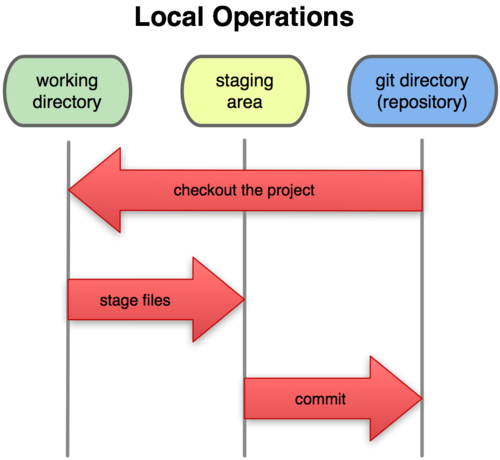
\includegraphics[scale=1.0]{git_local_ops.png}

\section{Сравнение на функционално ниво}
  \begin{tabular} { | l | p{22 mm} | p{21 mm} | p{14 mm} | p{17 mm} | p{34 mm} |}
  \multicolumn{6}{c}{Сравнение на разгледаните SCM} \\
  \hline
  Система     & Интерактивeн commit & Потребителят избира mergetool & Атомарeн commit & Промените са на ниво & Схема на ревизиите \\
  \hline
  CVS         & не                  & не                            & не              & файл                 & множество промени \\
  SVN         & не                  & да                            & да              & дърво                & множество промени \\
  Git         & да                  & да                            & да              & дърво                & копие на състоянието \\
  Mercurial   & да                  & да                            & да              & дърво                & множество промени\\
  \hline
  \end{tabular}

  \vspace{10 pt}

  % TODO(zori): Comment the workflows.
  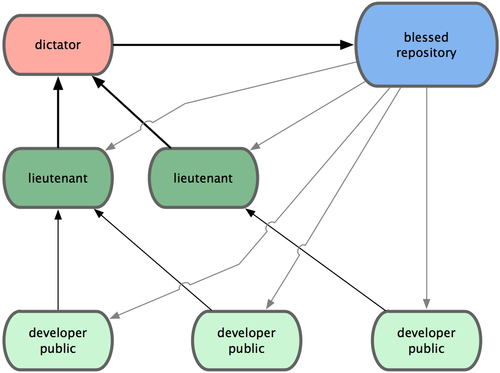
\includegraphics[scale=1.0]{benevolent_dictator_workflow.png}
  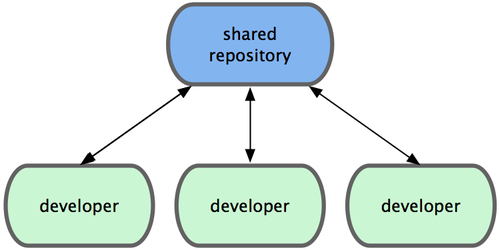
\includegraphics[scale=1.0]{centralized_workflow.png}

  \subsection{Предимства на централизираните системи}
    \begin{itemize}
      \item известни са на много голям брой програмисти
      \item изобилие от клиенти (графични, конзолни, web)
      \item много добра поддръжка в други приложения (IDE-та)
      \item проста концепция
      \item многократно доказани в разработване на големи, комерсиални проекти
      \item недостатъците и мерките за справяне с тях са добре известни
    \end{itemize}

  \subsection{Недостатъци на централизираните системи}
    \begin{itemize}
      \item създаването на ново repository изисква повече време и сървър
      \item при проблеми със сървъра целия процес на разработка не може да продължи
      \item включването на външен човек към екипа е тромаво и несигурно -- трябва да му се дадат привилегии за писане, което му дава неограничени права. Това е особено неприятно при проектите с отворен код, които разчитат най-вече на доброволци
      \item основните операции са в пъти по бавни от еквивалентите им при дистрибутираните системи
      \item при повечето централизирани системи няма утвърден начин за защита на кода от злонамерени и непреднамерени промени
      \item създаването на разклонения и сливането им е бавен, сложен, неефективен и за това избягван процес
    \end{itemize}

  \subsection{Предимства на дистрибутираните системи}
    \begin{itemize}
      \item Позволяват ефективна работа дори когато потребителите не са
      свързани в мрежа.
      \item Включването в проект е лесно - не изисква позволение за писане от
      привилегировани потребители.
      \item Използването за лични проекти е лесно и удобно. Подходящо за
      началните фази на проект, когато потребителите все още нямат нищо готово
      за публикуване.
      \item Не се създава единична централизирана контролираща система, която
      да създаде проблем в случай на срив. Всяко работно копие на базата може
      да служи за отдалечен backup на базата и историята на промените ѝ,
      намаляващо риска от загуба на данни.
      \item Все пак се позволява централизиран контрол когато е необходимо да
      се издаде официална версия на проекта.
      \item Повечето операции са много по-бързи отколкото в централизираните
      системи, тъй като не използват мрежата.
      \item Създаването на ново repository е изключително лесен и бърз процес.
      Това прави дистрибутираните системи много удобни за малки проекти.
      \item Разклоняването и сливането е естествен и утвърден процес. Това
      означава, че програмистите ще са по-склонни да започват експериментални
      промени от колкото при централизирано repository.
    \end{itemize}

    \paragraph{Отворени системи}
      Дистрибутираните VCS са подходящи за използване от отворени системи заради:
      \begin{itemize}
        \item \texttt{независимите разклонения}
        \item \texttt{лесното сливане на отдалечените хранилища}
      \end{itemize}

      При отворените системи:
      \begin{itemize}
        \item Всяко разклонение практически се имплементира като работно копие. Сливанията се извършват чрез размяна на patch-ове между отделните разклонения.
        \item Програмистите имат по-голяма готовност да създават нови версии на проекта когато е необходимо. Всъщност работното копие на хранилището само по себе си е потенциална нова версия. В случай, че неразбирателствата се изгладят сливането на кода в едно е лесно.
        \item Възможно е да се вземат само отделни промени (cherry-picking) подбрани от различни потребители.
        \item Не е задължително да съществува оригинално, отправно и единствено вярно копие на базата с код. Вместо това съществуват множество работни копия. В този смисъл е лесно да се създадат и множество ``централни'' хранилища.
        \item Код от отделните хранилища се слива на базата на т.нар. ``мрежа на доверието'' (web of trust). Исторически е доказано, че това подобрява качеството на кода.
      \end{itemize}

  \subsection{Недостатъци на дистрибутираните системи}
    \begin{itemize}
      \item начина на работа на дистрибутираните хранилища е по-сложен, което
      води и до по-сложен интерфейс на инструментите за работа с тях
      \item в момента дистрибутирания подход не е набрал голяма популярност,
      затова в нов проект трябва да се инвестира повече време за обучение на
      екипа
      \item съществуват системи за разработка (IDE) в които не са
      имплементирани разширения за комуникация с дистрибутирани repository-та
      \item Първоначалното клониране на хранилището на локалната машина
      е по-бавно в сравнение с централизираните системи, тъй като се копират
      всички разклонения с цялата им история.
      \item Липсват механизми за заключване, каквито традиционно са част от
      централизираните системи. Това е важно при двоични файлове, които не
      подлежат на сливане, например изображения.
    \end{itemize}

\section{Заключение}

%%%%%% End of document (EOD)
\newpage

\begin{thebibliography}{99}
  \bibitem{sccs} \url{http://sccs.berlios.de/}
  \bibitem{rcs} \url{http://www.gnu.org/software/rcs/}
  \bibitem{cvs} \url{http://savannah.nongnu.org/projects/cvs}
  \bibitem{svn} \url{http://subversion.apache.org/}
  \bibitem{git} \url{http://git-scm.com/}
  \bibitem{mercurial} \url{http://mercurial.selenic.com/}
  \bibitem{hg-design} \url{http://mercurial.selenic.com/wiki/Design}
  \bibitem{hg-bts} \url{http://mercurial.selenic.com/wiki/Design}
  \bibitem{sha1} \url{http://en.wikipedia.org/wiki/SHA-1}
  \bibitem{deflate} \url{http://en.wikipedia.org/wiki/DEFLATE}
  \bibitem{git-bottom-up} \url{http://ftp.newartisans.com/pub/git.from.bottom.up.pdf}
\end{thebibliography}

\end{document}
